%!TEX root = ../template.tex
%%%%%%%%%%%%%%%%%%%%%%%%%%%%%%%%%%%%%%%%%%%%%%%%%%%%%%%%%%%%%%%%%%%%
%% appendix3.tex
%% NOVA thesis document file
%%
%% Chapter with ROS Setup
%%%%%%%%%%%%%%%%%%%%%%%%%%%%%%%%%%%%%%%%%%%%%%%%%%%%%%%%%%%%%%%%%%%%
\chapter{System Setup on ROS}
\label{app:ros_setup}

\section{Introduction}
\label{sec:ros_setup_introduction}

The Robot Operating System (ROS) is a flexible framework for writing robot software. It is a collection of tools, libraries, and conventions that aim to simplify the task of creating complex and robust robot behavior across a wide variety of robotic platforms.

There are three core components that provide the robust environment for robotic development. These are its communication infrastructure at the low level; a set of robot-specific features; and some tools that ease the development process and debugging.

On the communication side we have message passing, message recording and playback, remote procedure call, and a distributed parameter system.

The robot-specific features are: standard robot messages; robot geometry library; robot description language; preemptable remote procedure calls; pose estimation, localisation and navigation; and diagnostics.

Regarding the tools, \gls{ros} comes with three powerful tools. It comes with command-line tools which give full control of the whole system, from compilation to code execution. Another tool is RViz which provides general purpose, three-dimensional visualisation of many sensor data types and any URDF-described robot. Finally, it also comes with rqt which is a Qt-based framework for developing graphical interfaces for the robot.

\section{Robot Setup}
\label{sec:ros_setup_robot}

This section describes how the robotic system integrates with \gls{ros}. It starts with the \gls{fci} components installation process. Then goes to communication network setup, followed by an overview of \textit{libfranka} and \textit{franka\_ros}.

\subsection{\gls{fci} Components Installation}
\label{subsec:ros_setup_robotic_system_integration_ros_installation}

 \textit{libfranka} and \textit{franka\_ros} can be installed on Windows and Linux. The computer \gls{os} used was linux, so linux installation instructions will be provided. For windows installation, refer to \cite{FrankaEmikaGmbH_fci_documentation}.\\

Official support is currently only provided to the following linux distributions:

\begin{itemize}
    \item Ubuntu 16.04 LTS Xenial Xerus and ROS Kinetic Kame
    \item Ubuntu 18.04 LTS Bionic Beaver and ROS Melodic Morenia (requires at least libfranka 0.6.0)
\end{itemize}

The \gls{os} used was Linux Mint Mate 19.2 64-bit. It is based on Ubuntu Bionic Beaver. All the needs are referenced to Ubuntu Bionic.

\subsubsection*{Installing franka\_ros}
\label{subsubsec:ros_setup_robotic_system_integration_ros_installation_franka_ros}

\textit{franka\_ros} can be installed from source or from repository. The easiest way to install is from repositories.

From linux command line, execute the following command \cite{FrankaEmikaGmbH_fci_documentation}:

\begin{verbatim}
    sudo apt install ros-melodic-libfranka ros-melodic-franka-ros
\end{verbatim}

% subsubsection robotic_system_integration_ros_installation_franka_ros

\subsubsection*{Installing libfranka}
\label{subsubsec:ros_setup_robotic_system_integration_ros_installation_libfranka}

\textit{libfranka} can also be installed from source or from repository. In this case, it is better to build from source. 
First any previous installation must be removed. To do it, run the following command \cite{FrankaEmikaGmbH_fci_documentation}:

\begin{verbatim}
    sudo apt remove "*libfranka*"
\end{verbatim}

Now, to build \textit{libfranka}, first install some dependencies:

\begin{verbatim}
    sudo apt install build-essential cmake git libpoco-dev libeigen3-dev
\end{verbatim}

Then, download the source code by cloning \textit{libfranka} from GitHub:

\begin{verbatim}
git clone --recursive https://github.com/frankaemika/libfranka
cd libfranka
\end{verbatim}

In the source directory, create a build directory and run CMake:

\begin{verbatim}
mkdir build
cd build
cmake -DCMAKE_BUILD_TYPE=Release ..
cmake --build .
\end{verbatim}

% subsubsection ros_setup_robotic_system_integration_ros_installation_libfranka

\subsubsection*{Installing real-time kernel}
\label{subsubsec:ros_setup_robotic_system_integration_ros_installation_realtime_kernel}

According to \cite{FrankaEmikaGmbH_fci_documentation}, "in order to control your robot using \textit{libfranka}, the controller program on the workstation PC must run with real-time priority under a PREEMPT\_RT kernel". An important notice is that NVIDIA binary drivers are not supported on PREEMPT\_RT kernels. This mean they must be deactivated before running in real mode.

Installing the real-time kernel is a more complex operation. The complete procedure is describe in \cite{FrankaEmikaGmbH_fci_documentation}. Visit the URL \url{https://frankaemika.github.io/docs/installation_linux.html#setting-up-the-real-time-kernel} for step by step instructions.

% subsubsection ros_setup_robotic_system_integration_ros_installation_realtime_kernel

% subsection ros_setup_robotic_system_integration_ros_installation

\subsection{\gls{fci} Communications Setup}
\label{subsec:ros_setup_robotic_system_integration_ros_comms_setup}

In order for the \gls{fci} to work, proper communication between the robot and the Host PC must be established. The connection between them should be direct, via Ethernet cable.

The Control and Host PC must be on the same network. For that, static IP addresses will be used. The IP configuration is provided on table \ref{tab:communicaton_setup_ips}.

\begin{table}[htbp]
    \caption[Control-Host PC network configuration values for static IP address and netmask.]{Control-Host PC network configuration values for static IP address and netmask.}
    \centering
    \begin{tabular}{l|c|c}
        \toprule
         & Host PC & Control \\
        \midrule 
         Address & 172.16.0.1 & 172.16.0.2 \\ 
         Netmask & 255.255.255.0 & 255.255.255.0 \\
         \bottomrule
    \end{tabular}
    \label{tab:communicaton_setup_ips}
\end{table}

Both IPs must be configured. To configure the Control's IP go to the browser and visit the URL \url{https://robot.franka.de/}, and follow these steps:

\begin{enumerate}
    \item On the top right corner, click the user name to open the menu.
    \item On the menu, select the \textbf{Settings} option (Fig. \ref{fig:panda_desk_top_menu}). A new page will open.
    \item On the Settings page, left menu, select \textbf{Network} option. The network options will appear.
    \item Change the IP address on the address text box on the right side of the screen (Fig. \ref{fig:panda_desk_settings_network_page}). Use the IP address from table \ref{tab:communicaton_setup_ips}.
    \item Uncheck the DHCP client checkbox on top of the address text box.
    \item Click the \textbf{Apply} button to save.
\end{enumerate}

\begin{figure}[htbp]
    \centering
	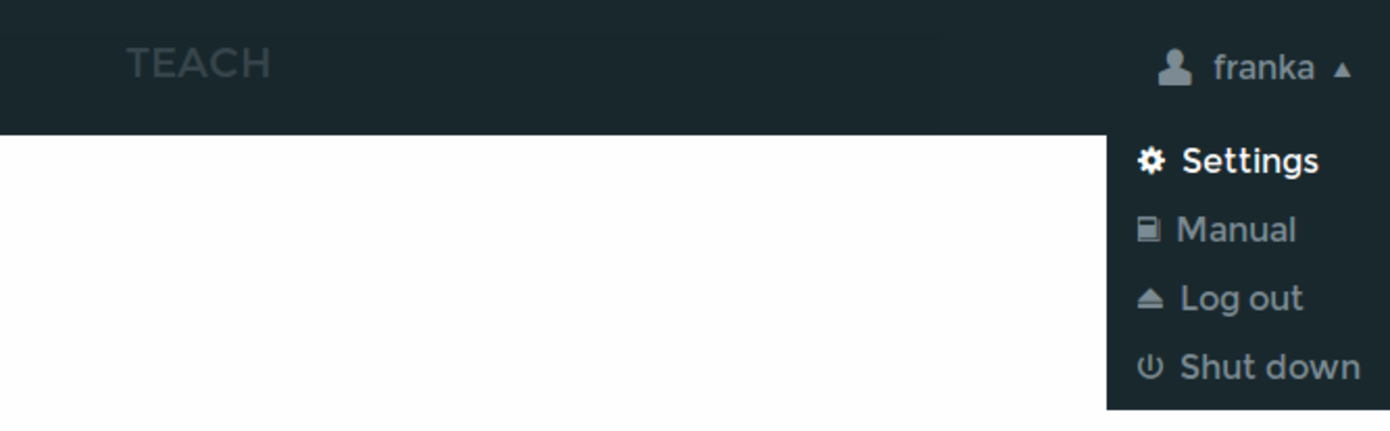
\includegraphics[width=\textwidth]{panda_desk_top_menu}
	\caption[Desk interface top right menu.]{Desk interface top right menu. Courtesy of Franka Emika GmbH and adapted from \cite{FrankaEmikaGmbH_fci_documentation}.}
	\label{fig:panda_desk_top_menu}
\end{figure}

To configure the host PC static IP, please refer to the specific \gls{os} instructions. On \cite{FrankaEmikaGmbH_fci_documentation}, within the \textbf{Getting Started} page, there is an example configuration for Ubuntu 16.04. You should use the IP address defined on table \ref{tab:communicaton_setup_ips}.\\

\begin{figure}[htbp]
    \centering
	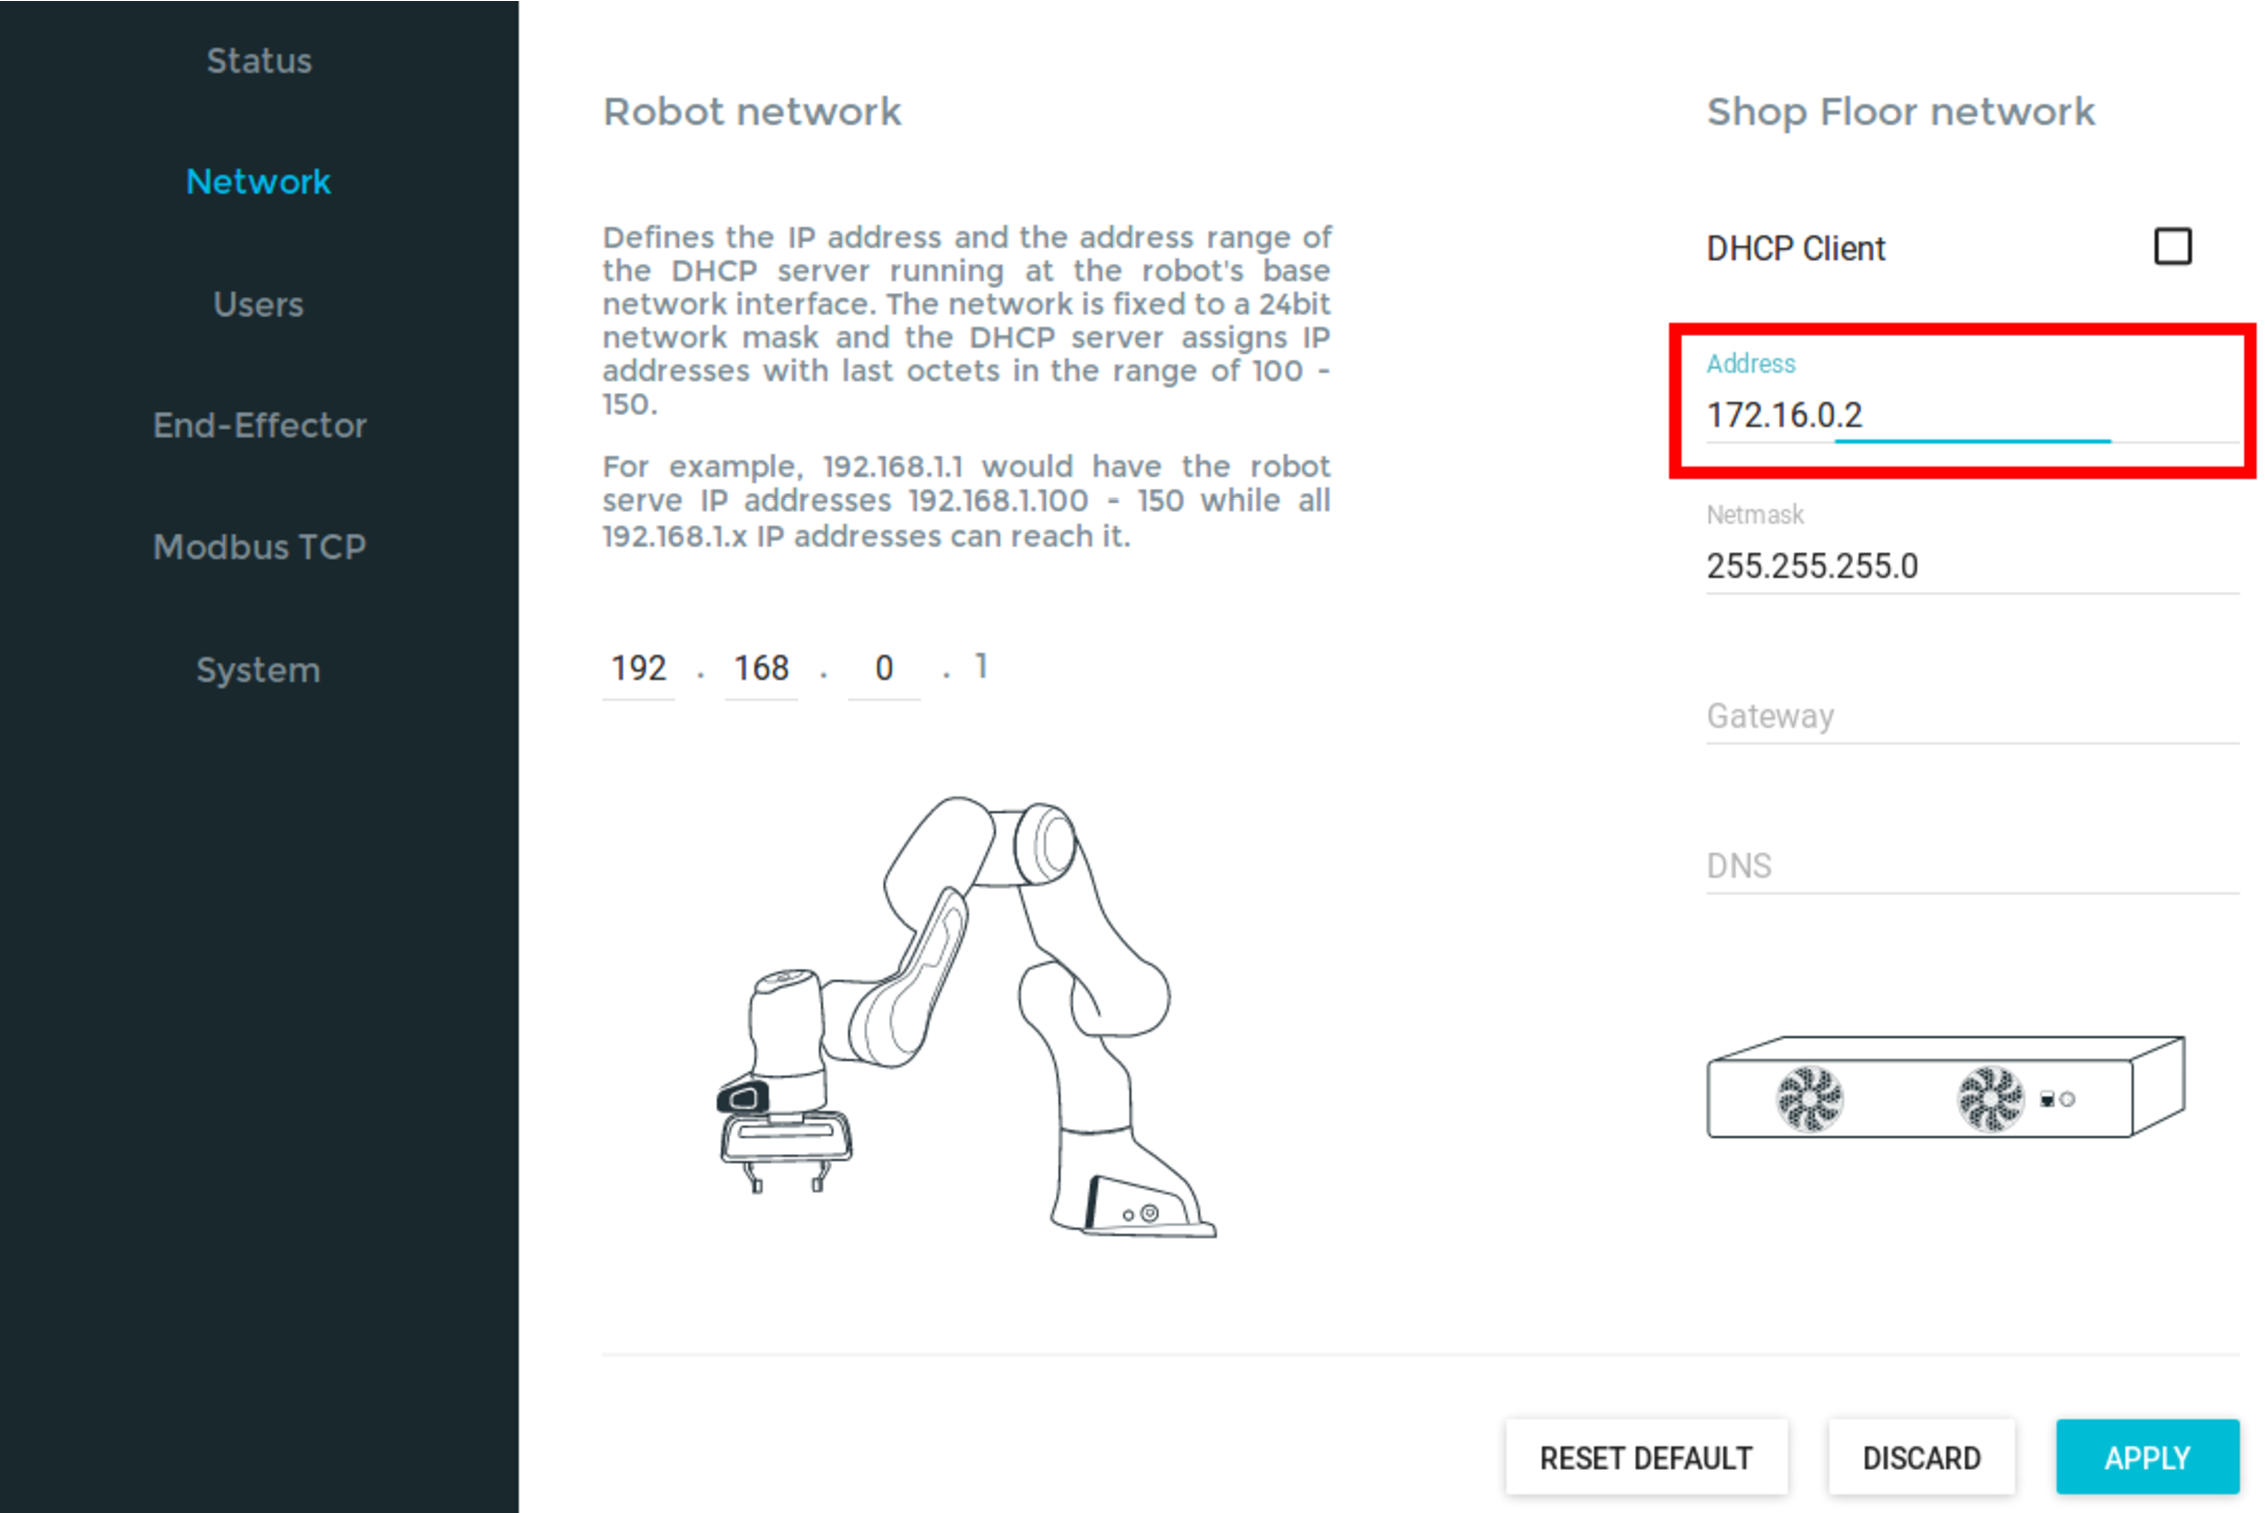
\includegraphics[width=\textwidth]{panda_desk_settings_network_page}
	\caption[Desk settings network page.]{Desk settings network page. The red box highlights the address text box where the new static IP for the control should be introduced. Courtesy of Franka Emika GmbH and adapted from \cite{FrankaEmikaGmbH_fci_documentation}.}
	\label{fig:panda_desk_settings_network_page}
\end{figure}

Finally, after all the configurations are done, the communication must be tested. To test the connection, first disable the fail safe locking system. Afterwards, go to \textit{libfranka}'s install folder and run the following command,

\begin{verbatim}
    ./examples/echo_robot_state <fci-ip>
\end{verbatim}

where \textbf{<fci-ip>} is the Control's static IP address. If everything is properly configured, the program will output the current robot state to the console. An example output is presented on Figure \ref{fig:panda_fci_network_config_example_output}.\\

\begin{figure}[htbp]
    \centering
	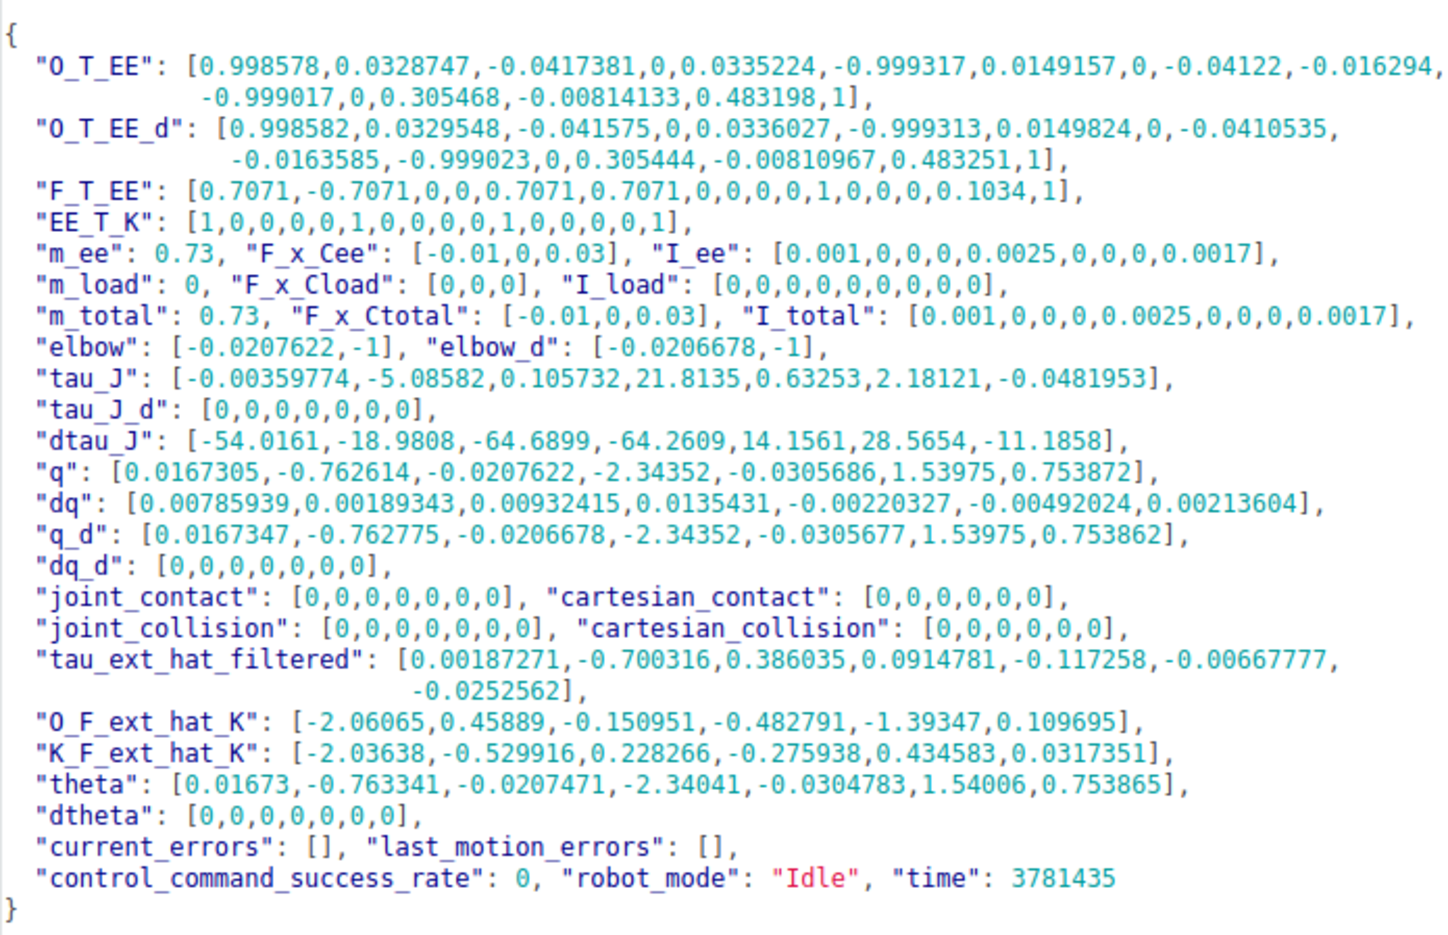
\includegraphics[width=\textwidth]{panda_fci_network_config_example_output}
	\caption[Desk settings network page.]{Proper network configuration test output example. Courtesy of Franka Emika GmbH and adapted from \cite{FrankaEmikaGmbH_fci_documentation}.}
	\label{fig:panda_fci_network_config_example_output}
\end{figure}

If any error happens at this point, please refer to the troubleshooting page from \cite{FrankaEmikaGmbH_fci_documentation}.

% subsection robotic_system_integration_ros_comms_setup

\subsection{libfranka}
\label{subsec:ros_setup_robotic_system_integration_ros_libfranka}

According to \cite{FrankaEmikaGmbH_fci_documentation}, \textit{libfranka} is "the C++ implementation of the client side of the FCI", and it "handles the network communication with Control". \textit{libfranka} also provides interfaces to:

\begin{itemize}
    \item execute non-realtime commands to control the Hand and configure Arm parameters.
    \item execute realtime commands to run your own 1 kHz control loops.
    \item read the robot state to get sensor data at 1 kHz.
    \item access the model library to compute your desired kinematic and dynamic parameters.
\end{itemize}

Figure \ref{fig:panda_fci_libfranka_overview} presents a schematic overview of \textit{libfranka}. This library acts as an interface for application development that needs to connect with the robot. \gls{fci} runs directly on Control and \textit{libfranka} is able to communicate with it via real-time and non real-time commands. There is also sensor data exchange to inform the upper layers of the robot state.

\begin{figure}[htbp]
    \centering
	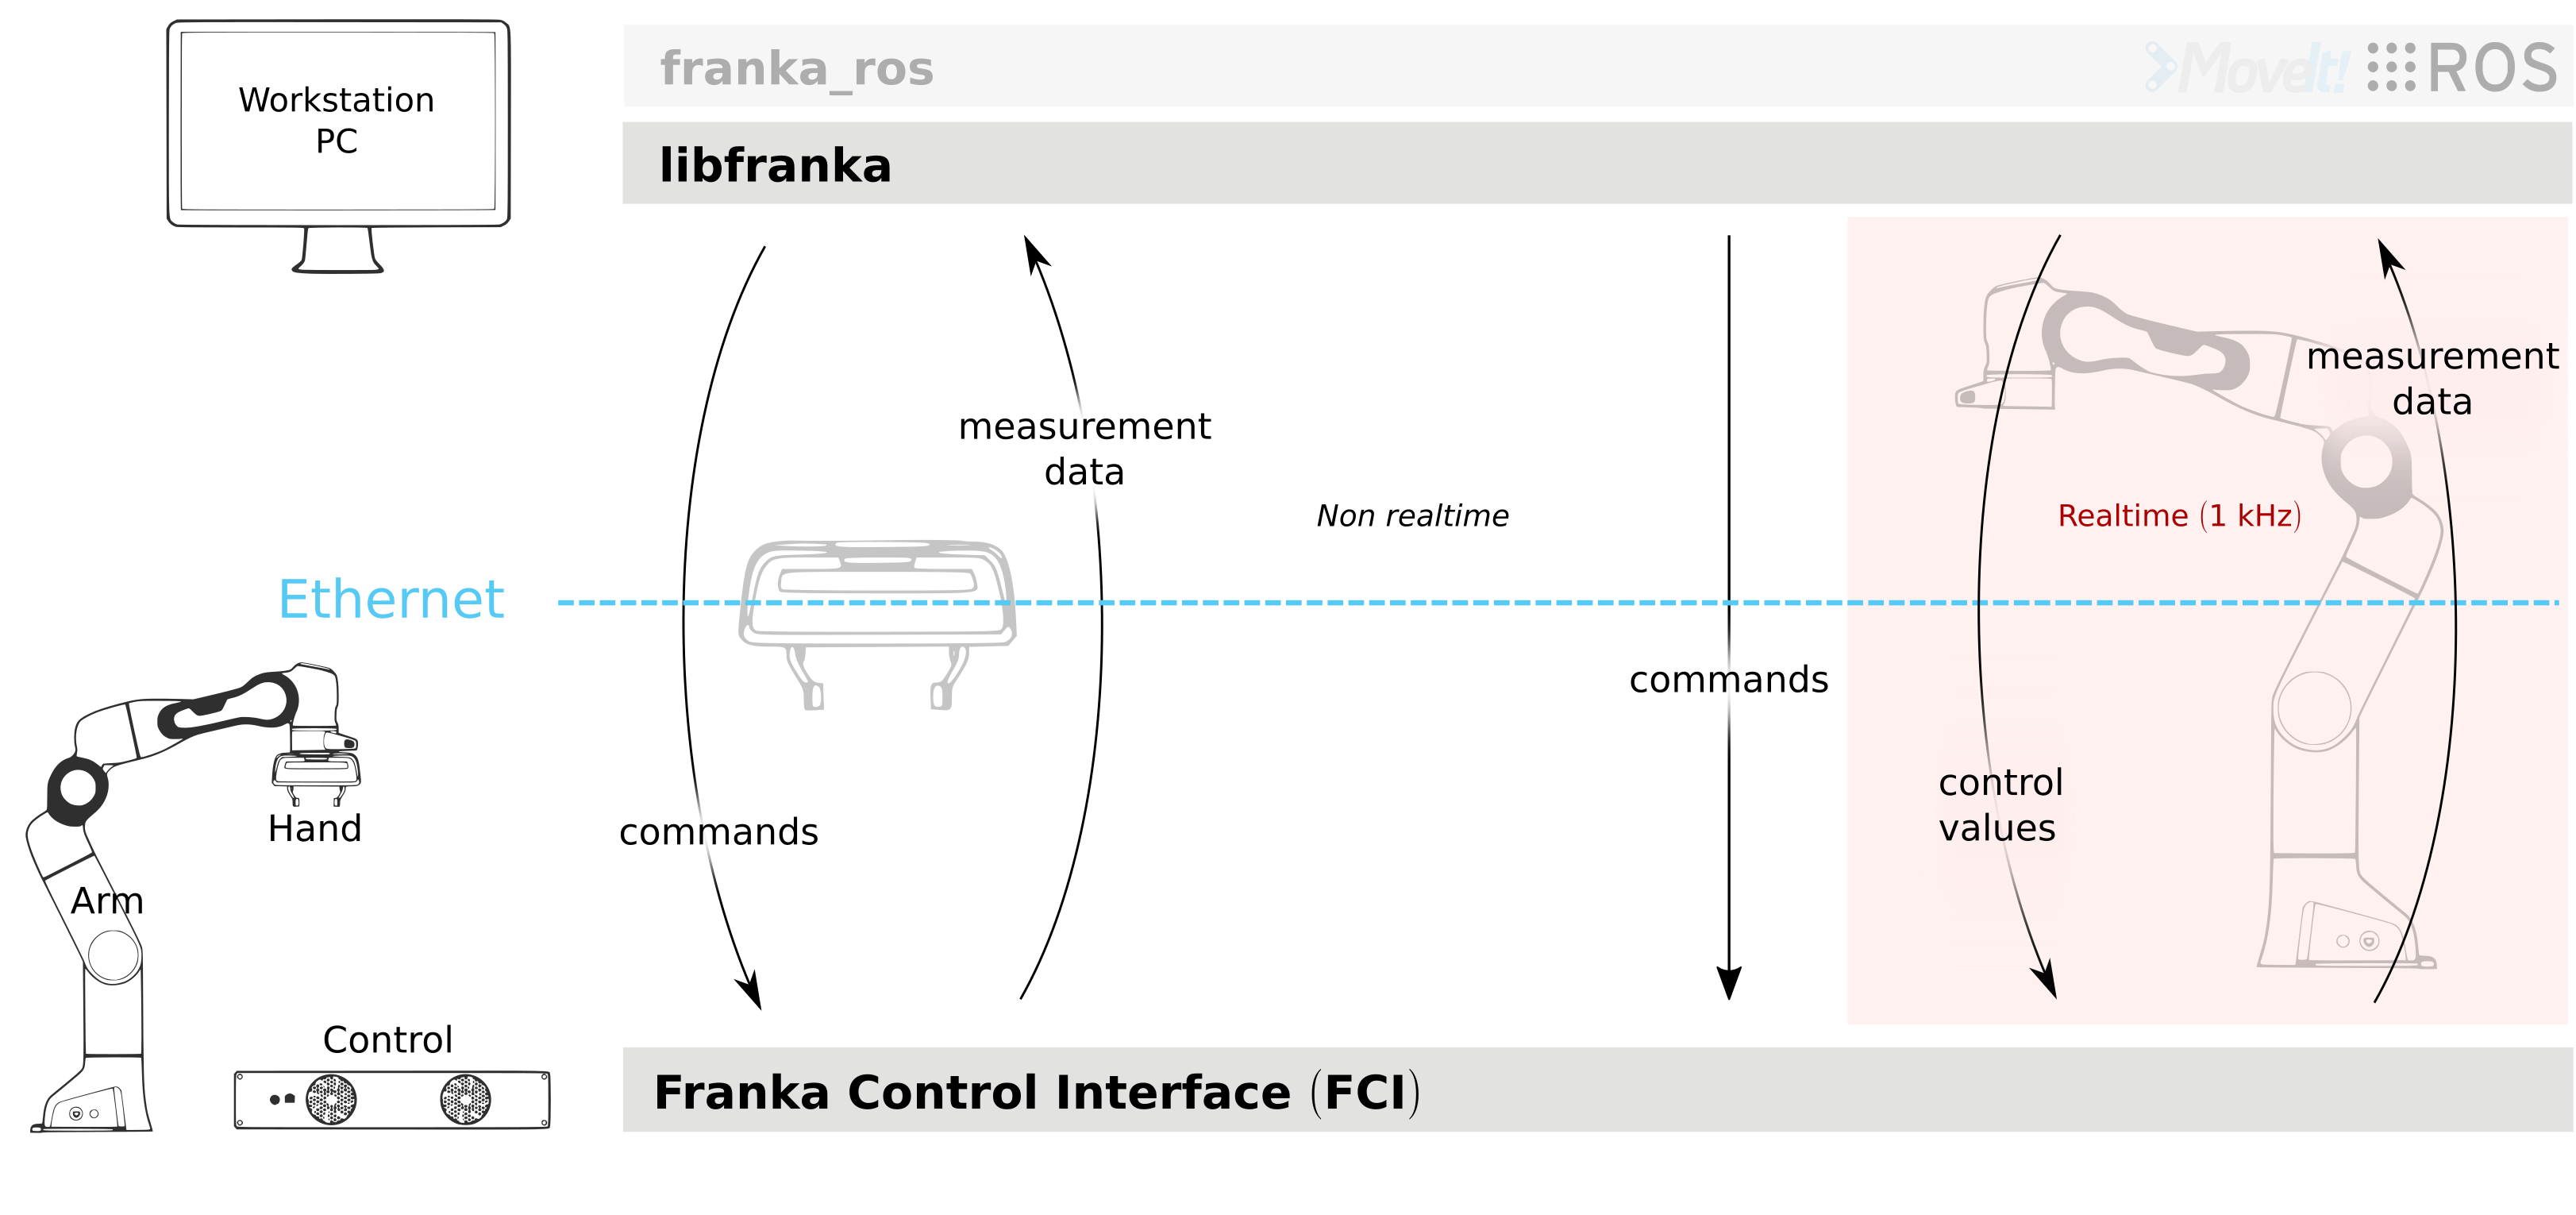
\includegraphics[width=\textwidth]{panda_fci_libfranka_overview}
	\caption[Schematic overview of \textit{libfranka}.]{Schematic overview of \textit{libfranka}. Courtesy of Franka Emika GmbH and adapted from \cite{FrankaEmikaGmbH_fci_documentation}.}
	\label{fig:panda_fci_libfranka_overview}
\end{figure}

For more information about \textit{libfranka} refer to \cite{FrankaEmikaGmbH_fci_documentation}.

% subsection ros_setup_robotic_system_integration_ros_libfranka

\subsection{franka\_ros}
\label{subsec:ros_setup_robotic_system_integration_ros_franka_ros}

\textit{franka\_ros} is built on top of \textit{libfranka} and is a set of \gls{ros} packages that integrate \textit{libfranka} into \gls{ros} and \gls{ros} Control. The packages provided by \textit{franka\_ros} are (see also Fig. \ref{fig:panda_fci_frankaros_overview}):

\begin{itemize}
    \item franka\_description
    \item franka\_gripper
    \item franka\_hw
    \item franka\_control
    \item franka\_visualization
    \item franka\_example\_controllers
    \item franka\_msgs
    \item panda\_moveit\_config
\end{itemize}

\begin{figure}[htbp]
    \centering
	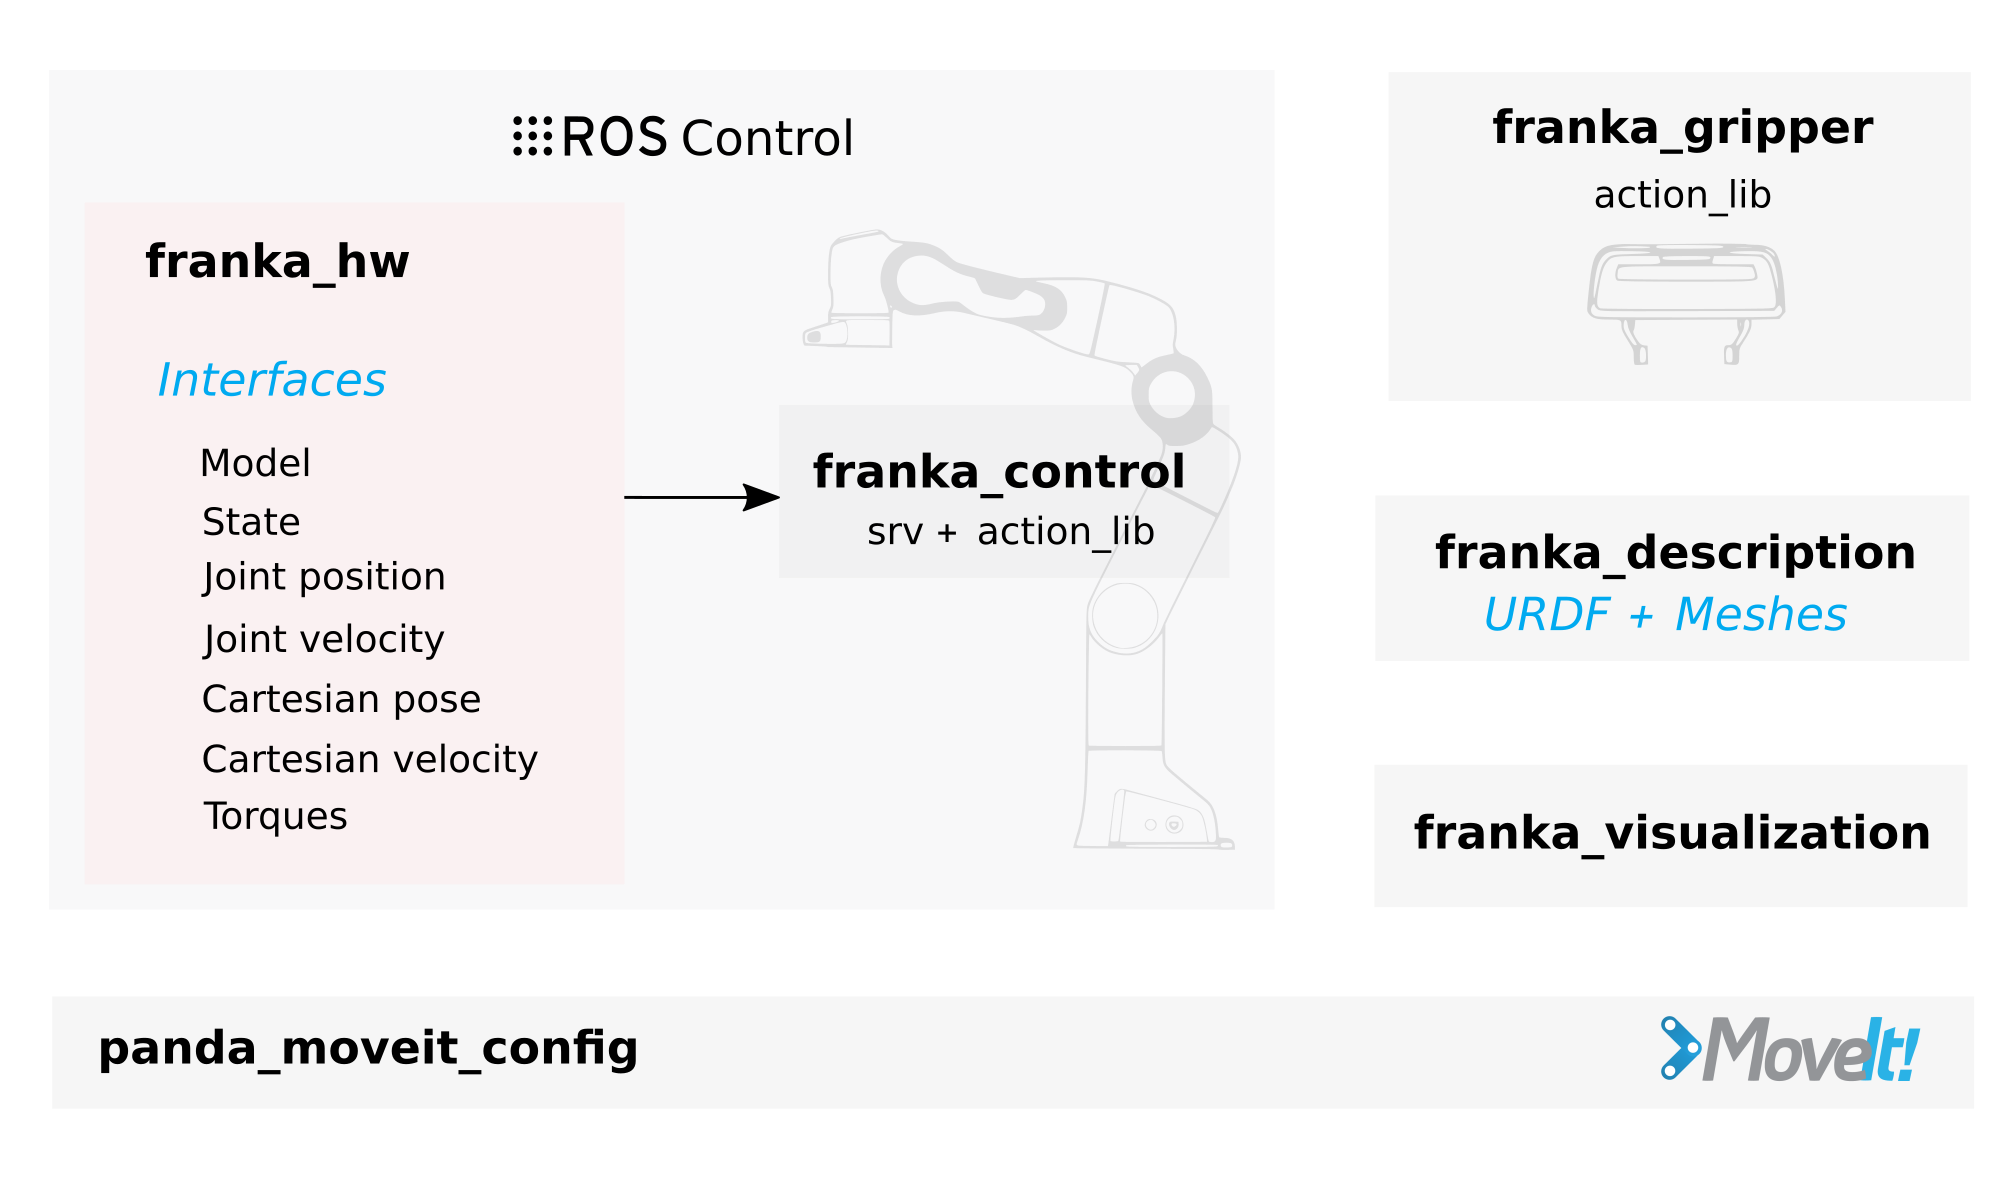
\includegraphics[width=\textwidth]{panda_fci_frankaros_overview}
	\caption[Schematic overview of \textit{franka\_ros} packages.]{Schematic overview of \textit{franka\_ros} packages. Courtesy of Franka Emika GmbH and adapted from \cite{FrankaEmikaGmbH_fci_documentation}.}
	\label{fig:panda_fci_frankaros_overview}
\end{figure}

\subsubsection*{franka\_description}
\label{subsubsec:ros_setup_robotic_system_integration_ros_franka_ros_franka_description}

This package contains the Panda Arm and Hand description in terms of "kinematics, joint limits, visual surfaces and collision space" \cite{FrankaEmikaGmbH_fci_documentation}. This allows the robot to be correctly visualized on RViz during operation. These descriptions will also be important for Gazebo simulation with only a few updates.

% subsubsection ros_setup_robotic_system_integration_ros_franka_ros_franka_description

\subsubsection*{franka\_gripper}
\label{subsubsec:ros_setup_robotic_system_integration_ros_franka_ros_franka_gripper}

This package implements a \gls{ros} node for interfacing a gripper from \gls{ros}. This allows the user to control Hand with \gls{ros} commands. The node publishes the state of the gripper and also provides several action servers.

% subsubsection ros_setup_robotic_system_integration_ros_franka_ros_franka_gripper

\subsubsection*{franka\_hw}
\label{subsubsec:ros_setup_robotic_system_integration_ros_franka_ros_franka_hw}

According to \cite{FrankaEmikaGmbH_fci_documentation}, franka\_hw package contains "the hardware abstraction of the robot for the ROS control framework based on the libfranka API".

% subsubsection ros_setup_robotic_system_integration_ros_franka_ros_franka_hw

\subsubsection*{franka\_control}
\label{subsubsec:ros_setup_robotic_system_integration_ros_franka_ros_franka_control}

This package provides two \gls{ros} nodes, \textbf{franka\_control\_node} and \textbf{franka\_combined\_control\_node}, which are hardware nodes for \gls{ros} Control. "They provide a variety of \gls{ros} services to expose the full libfranka API in the \gls{ros} ecosystem" \cite{FrankaEmikaGmbH_fci_documentation}. 

% subsubsection ros_setup_robotic_system_integration_ros_franka_ros_franka_control

\subsubsection*{franka\_visualization}
\label{subsubsec:ros_setup_robotic_system_integration_ros_franka_ros_franka_visualization}

This package is used only for visualisation. It publishes the robot and gripper joint states for visualisation in RViz.

% subsubsection ros_setup_robotic_system_integration_ros_franka_ros_franka_visualization

\subsubsection*{franka\_example\_controllers}
\label{subsubsec:ros_setup_robotic_system_integration_ros_franka_ros_franka_example_controllers}

To introduce the user to the control capabilities of Panda, this package provides "a set of example controllers for controlling the robot via \gls{ros}. The controllers depict the variety of interfaces offered ... and according usage" \cite{FrankaEmikaGmbH_fci_documentation}. To ease the controllers testing, each example comes with "a stand-alone launch file that starts the controller ... and visualizes it" \cite{FrankaEmikaGmbH_fci_documentation}.

% subsubsection ros_setup_robotic_system_integration_ros_franka_ros_franka_example_controllers

\subsubsection*{franka\_msgs}
\label{subsubsec:ros_setup_robotic_system_integration_ros_franka_ros_franka_msgs}

This package "contains message, service and action types that are primarily used by the packages franka\_hw and franka\_control to publish robot states or to expose the libfranka API in the \gls{ros} ecosystem" \cite{FrankaEmikaGmbH_fci_documentation}.

% subsubsection ros_setup_robotic_system_integration_ros_franka_ros_franka_msgs

\subsubsection*{panda\_moveit\_config}
\label{subsubsec:ros_setup_robotic_system_integration_ros_franka_ros_panda_moveit_config}

This package provides integration with \gls{ros} MoveIt!.\\

% subsubsection ros_setup_robotic_system_integration_ros_franka_ros_panda_moveit_config

% section ros_setup_robot

\section{Camera Setup}
\label{sec:ros_setup_camera}

This sections describes how to integrate the Intel\textregistered RealSense\texttrademark{} D415 depth camera into \gls{ros}. It starts with the installation process and follows with some custom setup and usage.

\subsection{Camera Installation}
\label{subsec:ros_setup_camera_installation}

The Intel\textregistered RealSense\texttrademark{} D400 product family \gls{sdk} comes with a port to \gls{ros}, consisting of two packages. These packages, \textit{realsense2\_camera} and \textit{realsense2\_description} are responsible for handling the data streams and making them available through \gls{ros} topics and defining the camera model for visualisation.\\

To install, we need to download the packages from RealSense-ROS github page at \url{https://github.com/IntelRealSense/realsense-ros/releases}. The release used was build v2.33.1.

The package folder should then be copied to \gls{ros} catkin workspace. Once there, just run the following commands on the terminal:

\begin{verbatim}
cd catkin_ws
catkin_make
\end{verbatim}

% subsection ros_setup_camera_installation

\subsection{Camera Customisation and Usage}
\label{subsec:ros_setup_camera_customisation_usage}

The \textit{realsense2\_camera} package comes with several launch files for several uses. The one we need to use is the \textbf{rs\_camera.launch}. It comes with many configuration options to customise the camera to our needs. The ones customised are the following:

\begin{itemize}
    \item camera: smalldrop/vision/camera/
    \item tf\_prefix: camera
    \item initial\_reset: true
    \item color\_width: 640
    \item color\_height: 480
    \item depth\_fps: 6
    \item color\_fps: 6
    \item enable\_pointcloud: true
    \item filters: pointcloud
    \item align\_depth: true
\end{itemize}

When running this launch file, it will start communication with the camera and stream the data via \gls{ros} topics:

\begin{itemize}
    \item /smalldrop/vision/camera/color/camera\_info
    \item /smalldrop/vision/camera/color/image\_raw
    \item /smalldrop/vision/camera/infra1/camera\_info
    \item /smalldrop/vision/camera/infra1/image\_raw
    \item /smalldrop/vision/camera/infra1/camera\_info
    \item /smalldrop/vision/camera/infra1/image\_raw
    \item /smalldrop/vision/camera/depth/camera\_info
    \item /smalldrop/vision/camera/depth/image\_raw
    \item /smalldrop/vision/camera/depth/color/points
\end{itemize}

% subsection ros_setup_camera_customisation_usage

% section ros_setup_camera

\section{Custom Code Structure}
\label{sec:ros_setup_custom_code}

All the code for this thesis is available on github: \url{https://github.com/blackchacal/smalldrop}. The whole code base is contained inside a \gls{ros} metapackage called \textit{smalldrop}. Within this metapackage, there are several other packages for specific tasks. The packages are:

\begin{itemize}
    \item \textit{smalldrop}: Project metapackage.
    \item \textit{smalldrop\_bioprint}: Responsible for controlling the whole system.
    \item \textit{smalldrop\_robot\_arm}: Responsible for the robot arm control for the real robot and Gazebo simulation.
    \item \textit{smalldrop\_msgs}: Responsible for declaring all messages, services and actions for the project.
    \item \textit{smalldrop\_rviz}: Responsible for handling rviz configurations and visualisation displays.
    \item \textit{smalldrop\_teleoperation}: Responsible for providing an interface for remote controllers for teleoperation. It provides a standard remote controller (Space Mouse Compact from 3Dconnexion).
    \item \textit{smalldrop\_toolpath}: Provides cartesian and joint path/trajectory planners.
    \item \textit{smalldrop\_state}: Responsible for declaring exceptions and provides a SystemState class that has general publishers and subscribers to be used by the other packages.
    \item \textit{smalldrop\_segmentation}: Responsible for providing wound segmentation algorithms for co-manipulation or camera segmentation.
    \item \textit{smalldrop\_vision}: responsible for controlling the camera.
\end{itemize}

As dependencies, there are the following packages or metapackages:

\begin{itemize}
    \item \textit{franka\_ros}
    \item \textit{realsense-ros}
    \item \textit{realsense\_gazebo\_plugin}
\end{itemize}

% section ros_setup_custom_code